\chapter{Placement strategies in commercial integrated titles}\label{placement}

While \chapref{overview} already provided an overview over the design of text elements and their translation in film in general, this chapter will focus on the \isi{placement} strategies of commercially-used integrated titles – how they came into existence, what the critics and audiences thought, and, most importantly, what \isi{placement} strategies are used frequently.\footnote{Parts of this chapter are also published in the article „Placement strategies for integrated titles – Based on an analysis of existing strategies in commercial films“ (Fox 2017) in a special issue of inTRAlinea (see \url{http://www.intralinea.org/specials/building_bridges} [2017--12--20]).} The goal is to create a basic set of strategies for the creation of the titles used in the study as well as to draft a recommendation for rules and strategies that can be used for the creation of integrated titles in general.

The analysis is product-based and was conducted by taking screenshots (of static titles) and short clips (of animated titles) from a selection of films. The first selection of three films is a sample analysis based on several criteria: The films are in English and offer subtitles that are placed on individual horizontal positions as illustrated in the ITC guidelines and by Karamitroglou, they are state-of-the-art by being released on BD and not older than 2010. As the existence of these ‘partially’ integrated titles is not listed as a specific characteristic, there is no way of creating a complete list of films that offer this feature. Therefore, the chosen films can only be a convenience sample. However, as they reflect the discussed guidelines for SDH in \sectref{sec:1.2.3}, they can be seen as representative of this recent resurrection of supposedly outdated rules, and there should be little variation, irrespective of the number of films.

The sample for the second part of this analysis consists of – to the investigator’s best knowledge – all examples of English films released between 2000 and 2015 that contain integrated titles that translate an \isi{additional language} into English as well as the so far only known film that made use of integrated titles throughout the whole length of the film, translating Russian into English. Contrary to the partially integrated SDH, there are no pre-existing guidelines or rules these integrated titles are based on. Therefore, all known examples were included in the sample analysis to reflect the state-of-the-art as accurately as possible while being able to exclude rare strategies due to their lower frequency.

Therefore, the following analysis takes into account two groups: Integrated titles for the hearing-impaired audience with only horizontal displacement (‘partially integrated titles’) and integrated titles targeted mainly at hearing audiences with the subcategories ‘partial translation’ and ‘complete translation’. The \isi{placement} strategies used in these films are analysed concerning their frequency and possible shortcomings. The most frequent strategies are then summarised in a first basic set of \isi{placement} strategies that forms the basis for the \isi{placement} of the titles in the present study. Their evaluation will show whether this set can later become the basis for a set of general guidelines for the creation of integrated titles.

\section{Partially integrated titles for the hearing-impaired audience}\label{sec:4.1}

Subtitles for the Deaf and Hard-of-Hearing have been around for quite some time and there have definitely been many attempts, both successful and unsuccessful, to add more information than the mere text can convey. Especially in television, SDH such as live subtitles often use colours to allow for an easier \isi{speaker identification}. Additionally, there have also been a few films that make use of it – for example \textit{The Dancer} (FR 2000), that (hardly by chance as the main protagonist is \isi{deaf}) combines the use of colour with a basic attempt to indicate the speaker by additionally aligning titles to the left and right in the bottom area:

\begin{figure}
\includegraphics[width=\textwidth]{figures/FIG16.jpg}
\caption{Speaker indication through colour and placement in \textit{The Dancer} (00:48:06 and 00:54:12).}
\label{fig:FIG16}
\end{figure}

Since then, not many subtitles have gone far beyond this. Therefore, it is even more gratifying that some BD releases offer SDH that actually follow the guidelines concerning \isi{speaker identification} through \isi{placement}: Titles that not only use the left and right corner as alternative positions but that are also placed in between and thus allow for a clearer \isi{speaker identification}. These partially integrated titles for a hearing-impaired audience can be found on some BDs, namely the following three most recent examples produced by Universal Pictures and Twentieth Century Fox (also the producers of the titles for \textit{Nochnoy Dozor} (“Night Watch”, RUS 2004), see \sectref{sec:4.2.1}):

\begin{table}
\begin{tabularx}{\textwidth}{p{11mm}p{12mm}lQQQ}
\lsptoprule
   Name &  Release &  Country &  Director &  Production studio(s) &  Main distributor\\
  \midrule 
 \itshape Jaws & (1975) 2012 & USA & Steven Spielberg & Zanuck/Brown Universal Pictures & Universal Pictures\\
\tablevspace
 \itshape Gone Girl & 2014 & USA & David Fincher & 20\textsuperscript{th} Century Fox\newline Regency Enterprises\newline TSG Entertainment & 20\textsuperscript{th} Century Fox\\
\tablevspace
 \itshape Ex Machina & 2015 & UK & Alex Garland & DNA Films Film4 & Universal Pictures\\
\lspbottomrule
\end{tabularx}
\caption{Overview of recent films with English partially integrated titles on the German BD releases}
\label{tab:TAB6}
\end{table}

BDs offering much more space\footnote{While DVDs offer 4.7 or 8.5 GB, BD offer up to 50~GB of space (see \url{http://www.audiogurus.com/learn/news/blu-ray-vs-dvd-upgrade/2616} [2015--12--30] and also \sectref{sec:2.2}).} might be one of the reasons of this recent development regarding SDH, but the integrated titles in films such as those discussed in the next chapter might have also played a central role in this process. Found to be representing the overall used \isi{placement} strategies in the respective films well, only the first three scenes of these films were analysed, resulting in slightly differing time spans. The differing number of titles, however, is more connected to the density of spoken dialogue in the films than the analysed time span. In the following, the three films are analysed and an overview of the derived \isi{placement} strategies is given.

\subsection{Sample analysis}\label{sec:4.1.1}

Being an already well-known film classic from 1975, the American production \textit{Jaws} tells the story of a gigantic white shark haunting the fictional island community of Amity that is finally killed by two residents and a marine scientist.\footnote{See \url{http://www.imdb.com/title/tt0073195/?ref\_=fn\_al\_tt\_1}, \url{http://www.blu-ray.com/movies/Jaws-Blu-ray/7547/}, and \url{http://www.jawsonbluray.com/} [2016--04--21].} The release on BD in 2012 brought a new layer to this special experience: The subtitles for the hearing-impaired are not placed solely in the centre of the bottom area but move around horizontally depending on the positions of speakers and noise sources.

The titles in \textit{Jaws} seem to follow the strategy of using the traditional position in the bottom-centre area as long as another position does not provide a better solution. Therefore, noise transcriptions and titles for off-screen speakers were placed about equally as often in the centre position as below a visible source in the image. For dialogues, however, titles were most likely placed below the speaker or below and in between multiple speakers. The combination of a speech act with a \isi{noise transcription} took place three times in the analysed time frame and was either placed under the speaker that also made the noise or assigned two individual positions to the two elements in the title (see \figref{fig:FIG17}).

\begin{figure}
\includegraphics[width=\textwidth]{figures/FIG17.jpg}
\caption{Speech and noise in one title but with individual positions in \textit{Jaws} (00:09:20)}
\label{fig:FIG17}
\end{figure}

\largerpage
Concerning the \isi{layout}, the titles use a simple \isi{sans-serif} \isi{typeface} in regular line width, coloured in white and with a thin black outline. While the titles are legible in front of a dark background, some titles in front of brighter image areas do not create a very strong contrast and are harder to read.

\textit{Gone Girl}, based on the thriller novel of the same name by Gillian Flynn and published in 2012, was released to the cinemas in 2014 and directed by David Fincher. The American film tells the story of Nick Dunne and his wife Amy who Nick reports as missing on their fifth wedding anniversary. Under pressure from media, police and relatives, Nick does not handle the situation very well and his strange behaviour makes more and more people suspect him to be the murderer of his wife.

The titles in \textit{Gone Girl} were most likely placed below the speaker respectively \isi{noise source} (see \figref{fig:FIG18}) or below and in between multiple speakers. As with \textit{Jaws}, it seems like the titles were placed in the traditional position whenever there was no visible benefit from placing it somewhere else. 

\begin{figure}
\includegraphics[width=\textwidth]{figures/FIG18.jpg}
\caption{Noise transcription placed below source (\textit{Gone Girl}, 00:02:52)}
\label{fig:FIG18}
\end{figure}

Overall, the titles in \textit{Gone Girl} offer good \isi{legibility} due to the clean, \isi{sans-serif} \isi{typeface} with a thin, black outline and titles close to the focus points. Even in front of a bright and diverse background the titles are comfortably readable.

The British production \textit{Ex Machina}, written and directed by Alex Garland, was released to the cinemas in 2015 and is a fiction thriller on the topic of artificial intelligence. The young programmer Caleb Smith wins an in-house competition and is invited to spend a week at the private retreat of his eccentric employer Nathan Bateman. He is asked to test the authenticity of what Nathan claims to be the first ever real artificial intelligence, but feels like there is more to it. The two first scenes analysed in \textit{Ex Machina} contain almost no titles placed in the traditional bottom-centre area of the screen. The sources of off-screen noises and the majority of noises with sources visible in the image were indicated through the title \isi{placement} (see \figref{fig:FIG19}). Titles for speakers outside the frame were placed almost exclusively below the \isi{focus point} in the image; the same goes for the majority of titles for visible speakers.

\begin{figure}
\includegraphics[width=\textwidth]{figures/FIG19.png}
\caption{Indication of noise source in \textit{Ex Machina} (00:06:06)}
\label{fig:FIG19}
\end{figure}

Despite the thin stroke width and the pale white tone, the \isi{typeface} and \isi{layout} used for the partially integrated titles in \textit{Ex Machina} offer a \isi{sufficient contrast} to be legible and reader-friendly – most likely due to the black outline and the wide character spacing of the \isi{sans-serif} \isi{typeface}.

\subsection{Shortcomings}\label{sec:4.1.2}

All in all, the titles in these films show that steps are taken to convey more information for the hearing-impaired audiences by making an effort to allow for an easier identification of speakers and noise sources. However, some problems could be identified in the sample and will be discussed here.

The main problem with the partially integrated titles for the hearing-impaired audience seems to be the creation of \isi{simultaneity} in dialogues that does not actually take place (see \figref{fig:FIG20}). The reason is most likely that these titles are still based on the traditional formatting and therefore contain speech acts of multiple speakers in single titles. Guidelines such as those by BBC clearly state that different speakers should not be captioned simultaneously “if they are not speaking at the same time” (\citealt{Ford_williams2009}:~12). All three analysed films created this \isi{alleged simultaneity} by displaying two consecutive speech acts at the same time. A solution would be to separate these titles and display the respective speech act when it actually takes place. Alternatively, the text for the second speaker can be delayed as an “add-on” (\citealt{Itc1999}:~14ff.) or “cumulative title” (\citeyear{Itc1999}:~14ff.) that coincides “with the onset of the second utterance, while the subtitle corresponding to the first utterance remains on screen” (\citeyear{Itc1999}:~14ff.), preserving the “natural relationship between speech onset and subtitle presentation” (\citeyear{Itc1999}:~14ff.). Both these solutions would not have to be performed by hand but can be achieved through algorithms such as the automatic splitting and pre-processing of subtitles files proposed by \citet{Hu2013}.

\begin{figure}
\includegraphics[width=\textwidth]{figures/FIG20.jpg}
\caption{Alleged simultaneity in \textit{Jaws} (00:09:12)}
\label{fig:FIG20}
\end{figure}

Another problem that should be addressed is the top area as a position for alternative \isi{placement}. This area is being proposed again and again (e.g. \citealt{Karamitroglou1998}, \citealt{Itc1999}) as suitable for the \isi{placement} of a title if the \isi{placement} in the traditional bottom area would result in it covering other relevant text or image elements. The problem is, while the bottom area is normally quite suitable as only few important image elements are placed here, this does not apply for the top area (especially in 16:9 film material; cf. \citealt{mercado2010}). And even if there is sufficient space and a title can be placed e.g. above a speaker (see \figref{fig:FIG21}), viewers might be less likely to notice a title being placed there. In \textit{Gone Girl}, one out of the 86 analysed titles was placed in the top area, and no title in the other two analysed examples \textit{Jaws} and \textit{Ex Machina}. That makes it quite unlikely for viewers to expect a title in that area. Their reaction might be too slow and the result could be irritation and a reduced \isi{enjoyment}. Another counter-argument might be directing the focus so far away from an obviously relevant element or area in the image (see the boardgame in \figref{fig:FIG21}).

\begin{figure}
\includegraphics[width=\textwidth]{figures/FIG21.jpg}
\caption{Title placed above the speaker in order not to cover the board game relevant for the dialogue (\textit{Gone Girl}, 00:02:38)}
\label{fig:FIG21}
\end{figure}

\newpage 
All in all, the partially integrated titles analysed in these films offer a good middle way in between traditionally placed subtitles and integrated titles. They should not, however, create \isi{simultaneity} where it does not belong and if possible avoid the top area of the screen if other areas in the image can provide \isi{sufficient contrast} and a logical \isi{placement}. While the \isi{layout} could still be improved, this approach offers easier access to the film and therefore possibly better entertainment. Yet, the partially integrated titles are only available in English on the German BDs. The German titles included in the release are placed traditionally and do not offer any of the benefits of their English counterparts.

\subsection{Derived placement strategies}\label{sec:4.1.3}

The placements used in the three SDH samples basically follow the supposedly outdated guidelines on SDH \isi{placement} that demand \isi{placement} close to the appropriate speaker or \isi{noise source} (\citealt{Itc1999}:~10) or below speakers (\citealt{Itc1999}:~13, \citealt{Jungst2010}:~129, \citealt{remael2007}:~31). In order to create categories for these placements, main groups according to the visible position of the speaker(s) or source of noise – based on both the human faces as almost irresistible “\isi{gaze} catchers” (\citealt{Lautenbacher2012}:142; cf. \citealt{Birmingham2008}) and the \isi{gaze} direction visible from the eyes (\citealt{Lautenbacher2012}:~142) – were created:

\begin{itemize}
\item Noise
\item Off-screen noise
\item Noise + Speaker
\item Off-screen speaker
\item 1+ Speaker(s)
\end{itemize}

Based on these categories on the number and visibility of speakers and noise sources, the following placements could be identified in the partially integrated titles for the \isi{deaf} and hard-of-hearing:

\begin{itemize}
\item Traditional (Bottom-centred)
\item Traditional (Top-centred)
\item Above speaker or \isi{noise source}
\item Below speaker or \isi{noise source}
\item Above focus (other than the speaker or \isi{noise source})
\item Below focus (other than the speaker or \isi{noise source})
\item Indication of \isi{noise source} outside the frame
\item Below \& In between
\item Next to speaker
\item Simultaneity
\end{itemize}

The listed strategies are now summarised following the distribution of visible speakers or noise sources. An example for the combination of speaker and noise can be seen in \figref{fig:FIG17}, an example of the indication of an \isi{off-screen noise} is illustrated in \figref{fig:FIG19}. The problem of \isi{simultaneity} is illustrated and discussed in the previous \sectref{sec:4.1.2}. The following additional strategies were derived from the sample: \figref{fig:FIG22} shows the identified positions for noise sources, \figref{fig:FIG23} shows the positions for off-screen speakers, and \figref{fig:FIG24} shows the identified positions for visible speakers.

\begin{figure}[p]
\frame{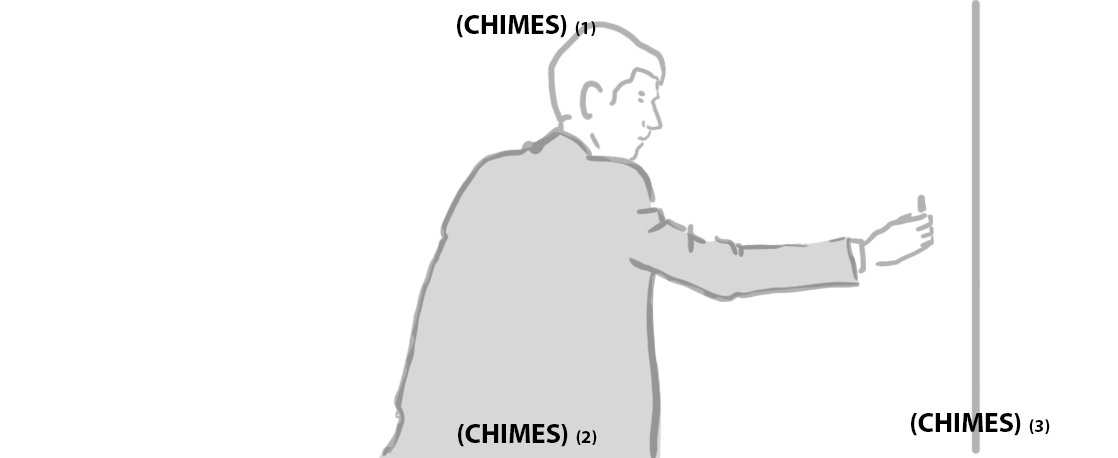
\includegraphics[width=\textwidth]{figures/FIG_22_nachbauen.png}}
\caption{Examples for identified positions for visible noise sources: 1) Traditional (top-centre), 2) traditional (bottom-centre), and 3) below noise source (sketch after a scene from \textit{Ex Machina}, 00:07:44).}
\label{fig:FIG22}
\end{figure}




\begin{figure}[p]
\frame{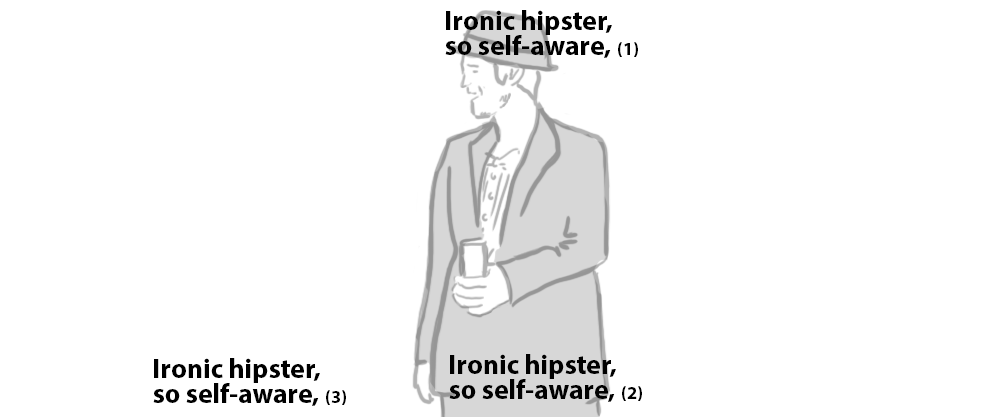
\includegraphics[width=\textwidth]{figures/FIG_23_nachbauen.png}}
\caption{Examples for identified positions for off-screen speakers: 1) Traditional (top-centre), 2) traditional (bottom-centre), and 3) below focus (sketch after a scene from \textit{Gone Girl}, 00:04:25).}
\label{fig:FIG23}
\end{figure}

\begin{figure}[p]
\frame{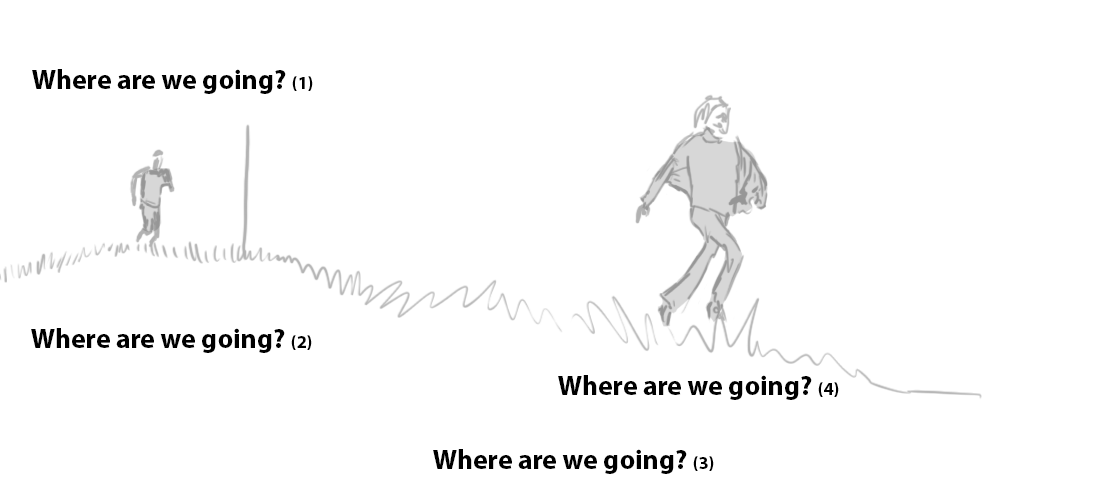
\includegraphics[width=\textwidth]{figures/FIG_24_nachbauen.png}}
\caption{Examples for identified positions for visible speakers: 1) Above speaker, 2) below speaker, 3) below \& in between/next to speaker, and 4) traditional (bottom-centre) (sketch after a scene from \textit{Jaws}, 00:02:31).}
\label{fig:FIG24}
\end{figure}

\begin{table}[p]
\small
\fittable{
\begin{tabular}{llrrrrrr}
\lsptoprule
 Visible speakers &  Placement strategy &  Jaws &  GG &  EM &  All &  \% &Film count\\
 \midrule 
 Noise & Traditional (bottom) & 11 & 5 & 2 & 18 & 5.61 & 3\\
 ~ & Traditional (top) & - & 2 & - & 2 & 0.62 & 1\\
& Below source & 10 & 5 & 5 & 20 & 6.23 & 3\\
% \tablevspace 
 Off-screen noise & Source indicated & - & - & 2 & 2 & 0.62 & 1\\
% \tablevspace 
 Noise + Speaker & Below source(s) & 3 & - & 2 & 5 & 1.56 & 2\\
% \tablevspace 
\multirow{2}{15mm}{Off-screen speaker} & Traditional (bottom) & 5 & 10 & 1 & 16 & 4.98 & 3\\
& Traditional (top) & - & 2 & - & 2 & 0.62 & 1\\
 ~ & Below focus & 2 & 2 & 8 & 12 & 3.74 & 3\\
% \tablevspace 
 1+ Speaker & Above speaker & - & 1 & - & 1 & 0.31 & 1\\
& Below speaker & 55 & 43 & 86 & 184 & 57.32 & 3\\
~ & Below \& In between & 12 & 7 & 6 & 25 & 7.79 & 3\\
~ & Traditional (bottom) & 6 & - & - & 6 & 1.87 & 1\\
~ & Next to speaker & 1 & - & 4 & 5 & 1.56 & 2\\
~ & Simultaneity & 6 & 9 & 8 & 23 & 7.17 & 3\\
\midrule
  &&  111 &  86 &  124 &  321 &  100.00 & \\
\lspbottomrule
\end{tabular}
}
\caption{Overview of the derived placement strategies for partially integrated titles}
\label{table:TAB7}
\end{table}

\clearpage 
The following \isi{placement} strategies could be identified in the analysed films \textit{Jaws}, \textit{Gone Girl} (GG), and \textit{Ex Machina} (EM). The following \tabref{table:TAB7} includes the individual counts per film as well as the summary of all three films.


For the \isi{noise transcription}, the traditional position at the bottom-centre and \isi{placement} below the source were used in the majority of the analysed situations and in all three films. As mentioned before, the top area can hardly be classified as suitable and was only used in two cases, accounting for less than 1\,\% of the overall titles. While the \isi{source indication} of an \isi{off-screen noise} was only used two times, it appears to be a suitable solution for a simply quite unlikely situation and can therefore be indicated by the \isi{placement} of the title (see \figref{fig:FIG19}). Concerning off-screen speakers, the traditional position and the position under the presumable main \isi{focus point} had the highest frequency. No placements were used that would indicate a speaker’s positions outside the frame, even though suitable situations were identified (see \figref{fig:FIG25} for an example).

\begin{figure}
\includegraphics[width=\textwidth]{figures/FIG25.png}
\caption{Title in the bottom-centre area even though it could have been placed closer to the right border indicating the speaker position outside the frame (\textit{Ex Machina}, 00:08:13)}
\label{fig:FIG25}
\end{figure}

While the strategies used for one and more speakers include a variety of solutions such as the \isi{placement} below a speaker and below and in between multiple speakers, there were also 23 titles (accounting for more than 7\,\% of titles in similar situations) that indicated the mentioned \isi{simultaneity} of two speech acts that actually did not take place in the audio channel (see \figref{fig:FIG20}).
 
\newpage 
Of the 111 titles analysed in the first two scenes of \textit{Jaws}, six titles were placed in the traditional position in the bottom-centre area in situations with one or more speakers. It is not comprehensible from the scenes why the titles were not placed below the speakers – \figref{fig:FIG26} for example shows sufficient place and contrast below the speaker but the titles in this scene remain in the bottom-centre area. As with the \isi{placement} in the top area, these solutions were only used in one of the three films and made up less than 2\,\% of all analysed titles. These two solutions will therefore not be taken into consideration for the final set of \isi{placement} rules.

\begin{figure}
\includegraphics[width=\textwidth]{figures/FIG26.jpg}
\caption{Title in the traditional position despite the sufficient space below the speaker (\textit{Jaws}, 00:07:34)}
\label{fig:FIG26}
\end{figure}

After the exclusion of suboptimal strategies – such as the \isi{placement} in the top area of the image and those creating \isi{simultaneity} – and strategies with low frequencies, a basic set of \isi{placement} strategies for partially integrated titles for the hearing-impaired can be derived from this analysis. Titles are placed below sources, foci and speakers, in between multiple speakers or in indication of a \isi{noise source} or speaker outside the frame (see \tabref{tab:TAB8}). While the speaker indication was not used in the analysed scenes, it makes sense to include it in order to add further information for a hearing-impaired audience.

\begin{table}
\begin{tabularx}{\textwidth}{XX}
\lsptoprule
 Visible speakers &  Placement strategy\\
 \midrule
 Noise & Traditional (bottom)\\
& Below source\\
& Source indication\\
\tablevspace
 Noise + Speaker & Below source(s)\\
\tablevspace
 Off-screen & Traditional (bottom)\\
& Below focus\\
\tablevspace
 1+ Speaker & Below speaker\\
& Below \& In between\\
& Speaker indication\\
\lspbottomrule
\end{tabularx}
\caption{Derived basic placement strategies from the sample analysis} 
\label{tab:TAB8}
\end{table}

More importantly than with the completely integrated titles that are discussed in the following section, positions outside the traditional (and therefore expected) areas should only be used if they are likely to lead to a better processing and experience than the bottom-centre area could offer, and not at all costs.

\newpage 
\section{Integrated titles for the hearing audience}\label{sec:4.2}

Tony Scott’s \textit{Man on Fire} might not be the first film ever to use a more creative approach on its subtitles for additional languages,\footnote{Early creative approaches include the “subtitles for people who don’t like subtitles” (DVD description, EMI Films, UK 1975) in \textit{Monty Python and the Holy Grail} with the text being taken from Shakespeare’s \textit{Henry IV, Part II} (cf. \citealt{Foerster2010}:~84), Jean-Luc Godard’s \textit{Vivre Sa Vie} (FR 1962) that features a main protagonist with subtitles instead of a voice (\citeyear{Foerster2010}:~84), Woody Allen subtitling unspoken thoughts in \textit{Annie Hall}, and subtitles in “Deperanto” that illustrate the language barrier in a foreign country (cf. \citealt{rozema2004}:~65--67).} but it seems to be the most frequently mentioned modern example (\citealt{Kofoed2011}; \citealt{mcclarty2012}; \citealt{romero-fresco2013}), followed quickly by the Russian film \textit{Nochnoy Dozor} with its creative subtitles for the English-speaking target audience. Together with \textit{Nochnoy Dozor}’s sequel \textit{Dnevnoy Dozor}\footnote{This film could not be analysed as it is even harder to come by than its prequel. It was released in the USA in 2007 with English titles by Twentieth Century Fox and Fox Searchlight Pictures.} (“Day Watch”, RUS 2006) and \textit{Slumdog Millionaire}, this “quartet of high-profile releases from Twentieth Century Fox and its specialty-film unit Fox Searchlight has initiated a radical, popular re-conception of the subtitle’s status in its previous distinction between inter- and intra-lingual contexts – as graphically additive captions and as linguistic translation” \citep{Kofoed2011}. They offer titles that are a “central aspect of the filmic mise-en-scène” \citep{Kofoed2011}\footnote{For a definition of mise-en-scéne, see \url{http://www.elementsofcinema.com/directing/mise-en-scene-in-films/} [2015--10--01].} and underline the fact that “subtitles as a graphic presence [are] inseparable from its medium as film” (\citealt{Egoyan2004}:~68). While \textit{Man on Fire} includes 219 integrated titles that translate from Spanish into English (compared to 1332 subtitles if watched with English subtitles, therefore accounting for approximately 16.44\,\% of the film’s dialogue), the English subtitled version of \textit{Nochnoy Dozor} offers a complete translation for the foreign English-speaking audience with integrated titles accounting for around 6.46\,\% of the overall subtitles. Therefore, two kinds of integrated titles can be identified here: Titles that are part of the original version of a film and translate an \isi{additional language} (cf. \textit{Man on Fire}, \textit{Slumdog Millionaire}), and titles that translate an entire film into another language for a foreign target audience (cf. \textit{Nochnoy Dozor}, \textit{Dnevnoy Dozor}).

\subsection{Sample analysis}\label{sec:4.2.1}

While the integrated titles for the hearing-impaired audience described in the previous chapter seem to be a fairly new development with recent examples only a few years old, the integrated titles as translation tool for an \isi{additional language} in an English film reach, as already stated, at least back to 2004 (\textit{Man on Fire}) and are often traced back to the very beginnings of text elements in film, namely intertitles (\citealt{mcclarty2012}:~136; \citealt{romero-fresco2013}:~205). Apart from \textit{Nochnoy Dozor}, the films discussed in this section were all produced in the USA. The following \tabref{tab:TAB9} represents the analysed sample.

\begin{table}[b]
\small
\begin{tabularx}{\textwidth}{L{18mm}L{11mm}@{\,}Q@{\,}QQp{15mm}}
\lsptoprule
 \bfseries Name &  Release &  Director &  Production studio(s) &  Main distributor &  Languages\footnote{The main language in the film is given in the first line, the additional, subtitled language in italics in the second line. As \textit{Nochnoy Dozor} was subtitled completely from Russian into English, only the source language is stated.}\\
 \midrule 
 \itshape Man on Fire & 2004 & Tony Scott & Warner Bros. International & Twentieth Century Fox & English \newline\textit{Spanish}\\
 \tablevspace 
 \itshape Nochnoy Dozor & 2004\newline   2006 & Timur Bekmambetov & Channel One & Twentieth Century Fox & Russian\\
 \tablevspace 
 \itshape Heroes \itshape (Episode 01) & 2006 & Tim Kring & Tailwind Productions & Universal Pictures & English\newline \textit{Japanese}\\
 \tablevspace 
 \itshape Slumdog Millionaire & 2008 & Danny Boyle & Celador Films Ltd. & Twentieth Century Fox & English \newline  \textit{Hindi}\\
 \tablevspace 
 \textit{Fast Five}\footnote{There 
  is also a small number of similar titles in the following films of the series (\textit{Fast \& Furious~6} [USA 2013], \textit{Fast \& Furious 7} [USA/JP 2015]). The same goes for further \textit{Heroes} episodes.
  } 
  & 2011 & Justin Lin & Original Film\newline  One Race Films, Dentsu & Universal Pictures & English\newline \textit{Portuguese}\\
 \tablevspace 
 \itshape Star Trek Into Darkness & 2013 & J.J. Abrams & Bad Robot & Paramount Pictures & English \textit{ Klingon}\\
 \tablevspace 
 \itshape John Wick & 2014 & Chad Stahelski\newline  David Leitch & 87Eleven & Lionsgate Entertainment & English\newline  \textit{Russian}\\
\lspbottomrule
\end{tabularx} 
\caption{Overview of the analysed films with integrated titles for an additional language}
\label{tab:TAB9}
\end{table}

 “Subtitles are boring” – this simple opinion stated by Tony Scott (Scott, interview\footnote{Interview with Tony Scott, performed by Daniel Robert Epstein for UGO in 2007, as quoted in \citet{Kofoed2011}.}) led to a new view on subtitles after decades of lacking interest from directors and producers. Without knowing that he would establish a new trend, if not even a future paradigm shift, he wanted the subtitles to be conceived as a “kind of character in the scene” (\citealt{Kofoed2011}).

Therefore, the American remake\footnote{Information on the 1987 original of the same name can be found here: \url{http://www.imdb.com/ title/tt0093489/} [2012--06--25]. Information on the remake: \url{http://www.imdb.com/title/tt0328107/} [2012--06--25].} \textit{Man on Fire} provides a variety of integrated and aesthetically pleasing titles. The film takes place in Mexico and tells the story of ex-legionnaire and soldier John Creasy. While he appears to have already given into his alcohol addiction, his best friend convinces him to take on a job as bodyguard for the 9-year-old Pita, the daughter of a rich married couple. Very slowly and hesitantly, a strong friendship develops and John seems to recover – until Pita is abducted and John seriously injured. When the handover of the ransom money fails and Pita is killed, John sets out to find the kidnappers. With the setting in Mexico, several words and phrases in the film are in Spanish. However, not only this spoken content is subtitled, but also some English statements – presumably to underline and intensify the corresponding content:
\begin{quote}
The traditional, translating purpose of the subtitle is directly questioned, as characters speaking in accented English are selectively subtitled, until even Denzel Washington’s mixed language dialogue is transcribed according to purely \isi{aesthetic} considerations during emotionally heightened scenes. This non-translative doubling of the dialogue with its textual equivalent marks a radical reconception of a text’s potential function in another otherwise typical Hollywood production, an inescapably heightened awareness and assertion of the visual nature of the subtitle. \citep{Kofoed2011}
\end{quote}

Another interesting aspect is the conscious \isi{placement} in the mise-en-scène or “within the shot’s depth of field, such that characters and objects may move before the subtitles, obscuring them from the reader’s \isi{gaze}” \citep{Kofoed2011}. In addition to several fading animations (see \figref{fig:FIG27}), a wide variety of kinetic effects was used to underline the active role of the titles in \textit{Man on Fire}. Concerning the \isi{layout}, the titles are rendered mostly in Franklin Gothic\footnote{See, for example, \url{https://typekit.com/fonts/franklin-gothic-urw} [2015--09--11]. Two other unidentified typefaces were used in a small number of titles, one of them resembling type printed in newspapers.} and well readable due to their \isi{sans-serif} and bold character that provides a good contrast to film image. They are “not confined to the top layer of the film, they have depth and perception” \citep{Vit2005}.

\begin{figure}
\includegraphics[width=\textwidth]{figures/FIG27.png}
\caption{Additional fading effect in \textit{Man on Fire} (01:03:18).}
\label{fig:FIG27}
\end{figure}


As mentioned before, the integrated titles in \textit{Man on Fire} (see \tabref{tab:TAB11}) account for approximately 16.44\,\% of titles needed to subtitle the complete film (219 out of 1332 titles). Titles for off-screen speakers were either placed quite traditionally in the bottom-centre area or close to focal points in the image. With one speaker visible in the image, the titles were mostly placed below him or her. About 19~titles were placed next to the speaker, even if there would have been space to indicate the \isi{speaking direction}, as it was done with 54~titles. Therefore, the most frequently used positions for one visible speaker were below the speaker or in \isi{speaking direction} (approximately 84\,\%). If there were at least two speakers visible, the titles were placed in between them. Only one title is placed below the person that is spoken to.


As stated above, another interesting feature of \textit{Man on Fire} is the use of titles not only for translation, but also emphasis of already English terms and statements (adding \isi{intralingual translation} to the otherwise \isi{interlingual} titles), which account for 17.35\,\% of the integrated titles (38 out of 219).

The reactions to \textit{Man on Fire} were mixed. While some critics celebrated the innovative titles as “small, visual victories that add charisma and personality to commonly bland and uninspiring subtitles” \citep{Vit2005}, others such as film critic Brian Gallagher refer to them as an example of “how NOT to do subtitles” \citep{Gallagher2004}. While \textit{Man on Fire} displays several \isi{aesthetic} types of text integration, it is not always comprehensible on what basis the present effect was chosen. Some titles are displayed word by word, corresponding to the actual speed of speech, while others are displayed in a whole or line by line, flicker, re-appear after a scene cut or move through the image. A smaller, but more comprehensive selection of effects might have had a stronger and more thoughtful impact.

Furthermore, these integrated titles seem to only be part of the English original version of the film. For the German DVD and BD releases, the titles were removed and replaced with traditional subtitles.

``Rejoice – subtitles have been freed!” With this exclamation, the Washington Post celebrated \textit{Slumdog Millionaire’s} titles when the film came to the cinemas in 2008 \citep{Beckman2008}. \textit{Slumdog Millionaire} tells the story of the young orphan adult Jamal who participates in the Indian version of “Who Wants to Be a Millionaire?” to find the love of his life. While the film was initially supposed to be completely in English, the British director Danny Boyle quickly realized that the child actors would not be able to deliver their lines credibly in English (\citeyear{Beckman2008}). He therefore decided to let them speak Hindi and promised Warner Independent\footnote{Later replaced by Fox Searchlight Pictures as main production studio.} “that the film would be even~more~exciting because of the subtitles” (\citealt{Beckman2008}; cf. \citealt{Kofoed2011}). He “came up with the idea to have the subtitles look more like the dialogue in comic books, which float depending on where the characters are positioned” \citep{Beckman2008}. According to McClarty, this “works to keep the audience engaged with the plight of the young boys” (\citeyear{mcclarty2012}:~143). The titles were also “placed within coloured \isi{caption} boxes” \citep{Kofoed2011}\footnote{Created by London-based \isi{title designer} Matthew Curtis.} and inspired not only by comic book captions but also the nontraditional subtitles of \textit{Nochnoy Dozor} (\citealt{Beckman2008}; \citealt{Kofoed2011}). The coloured boxes ensure both “visibility” (\citealt{mcclarty2012}:~143) and \isi{legibility} against the changing background and slightly resemble compositions on posters and in comic books. While traditional subtitling conventions often suggest black boxes (e.g. \citealt{Karamitroglou1998}), the “colour of the transparent box changes according to the colour scheme of the mise en scène” (\citealt{mcclarty2012}:~143) in \textit{Slumdog Millionaire}. The 202 integrated titles account for about 17.99\,\% of the film’s dialogue (out of approximately 1123 subtitles if watched with closed captions).

The Washington Post’s film critic Rachel Beckman described the titles in \textit{Slumdog Millionaire} as bouncing “around the screen in a rainbow of colors” \citep{Beckman2008} and “stylish and splashy and original. They’re liberated” (\citeyear{Beckman2008}). McClarty underlines the importance of these titles not only fulfilling “their linguistic, translational function” (\citealt{mcclarty2012}:~143) but “also fulfilling an equally important \isi{aesthetic} function through their colour and an affective function through their positioning in the heart of the on-screen action” (\citeyear{mcclarty2012}:~143). However, she notes that these titles rather allow for an “overall understanding of the situation and dialogue, rather than a word by word comprehension of each subtitle” (\citeyear{mcclarty2012}:~143) and also Romero-Fresco sees that “the translational role of these subtitles (and even their \isi{legibility}) often takes a back seat to their affective use of colour and position to advance plot and character development” (\citealt{romero-fresco2013}:~210). This discussion of the titles in \textit{Slumdog Millionaire} shows that decisions concerning the significance awarded to the translational function of the titles on the one hand and the \isi{aesthetic} and affective function on the other have a strong influence on the final product and translators and designers involved in the postproduction have to work hand-in-hand to achieve a good result.

\begin{figure}
\includegraphics[width=\textwidth]{figures/FIG28.jpg}
\caption{Indication of speaker outside the frame in \textit{Slumdog Millionaire} (00:34:49).}
\label{fig:FIG28}
\end{figure}

In addition to ignoring the \isi{layout} instructions of the traditional guidelines, the titles also lack periods at the end of the only or last sentence within a title. This might lead to irritation of the audience as it might not be clear whether the sentence was finished or will continue in a following title. The \isi{typography} is modest and makes use of a single \isi{typeface} with soft edges and a legible stroke width. The combination of \isi{typeface}, drop shadow and coloured box, however, might lead to a decrease in \isi{legibility}. From examples such as \figref{fig:FIG28}, it appears as if the \isi{image composition} was considered more important than indication of speaker or \isi{speech direction}, but then there are also titles that disturb the \isi{image composition} strongly even though better solutions would have been possible. While the \isi{placement} of the titles could be improved by decreasing the distance to the speakers and focus points, the overall \isi{layout} and especially the coloured boxes support the atmosphere and emotions in the respective scenes and most likely had a strong impact on the reception of \textit{Slumdog Millionaire}.

The American television show Heroes was produced and broadcast by NBC between 2006 and 2010.\footnote{Also taking into account its sequel \textit{Heroes Reborn} (USA 2015--2016) with a similar concept of integrated titles.} It consists of four seasons and its dubbed German version was broadcasted by the Swiss channel “SF zwei” and the German channel “RTL2”.\footnote{For further information, see \url{http://www.imdb.com/title/tt0813715/} [2015--10--02].} \textit{Heroes} tells the story of a group of people all over the world that developed supernatural abilities. While there seems to be no connection between the various stories, shared fate brings them together and everyone has to decide for themselves on which side of the fight for Earth’s future he or she will stand.

While almost all characters in \textit{Heroes} speak English, the Japanese friends Hiro and Ando speak their mother tongue at the beginning of the first season and only learn English bit by bit due to their continuous stay in the United States.\footnote{There is also a South American pair of siblings in the second season that speaks Spanish. However, the corresponding English subtitles were placed traditionally – the only noticeable difference is the yellow colour that might be intended to refer to their Southern origin or offers a better contrast to the often dark green image.} Thus, Hiro and Ando are the only characters in the first season to be subtitled. These titles were integrated into the image dynamically, seemingly on the basis of the \isi{placement} of speech bubbles in comics as Hiro is a huge fan of them and draws all his knowledge of supernatural abilities and other characters from them. The integrated titles in the first episode of the first season of \textit{Heroes} (see \tabref{tab:TAB11}) make up about 13.56\,\% of the film’s dialogue, accounting for 96 titles out of 708 in total. For speakers outside the frame, the titles were more frequently placed traditionally in the lower centre area of the screen or in an area providing a good contrast than as an indicator of \isi{speaking direction}. In the case of one visible speaker, the titles were most likely placed below this person, also accounting for over 53\,\% of all placed titles in \textit{Heroes} (Season 1, Episode 1; S01E01). For two or more speakers, the titles were often placed in the lower area, but in between the speakers, therefore allowing the viewer to read the titles while switching between the speakers of a conversation. Alternatively, if the frame offered enough space, the titles were placed in between the speakers faces (see \figref{fig:FIG29}).

\begin{figure}
\includegraphics[width=\textwidth]{figures/FIG29.png}
\caption{Title placed in between speakers during a dialogue in \textit{Heroes} S01E01 (00:14:12)}
\label{fig:FIG29}
\end{figure}

Overall, the first episode of the first season of \textit{Heroes} showcases many interesting \isi{placement} strategies and might include some of the first film material that was actually shot in a way that would provide space and \isi{sufficient contrast} to allow for the title \isi{placement} in the postproduction.

\textit{Fast Five} was released to cinemas in 2011 as a joint production between Original Film, One Race Films and Dentsu, distributed by Universal Pictures. Even though the screened version included 101 individually placed titles translating Portuguese conversations and statements into English, no mention of this can be found in critic’s reviews of the fifth part of the \textit{Fast \& Furious} series. In the film, the former cop Brian, his girlfriend Mia and her brother Dom fled the United States to Rio de Janeiro after they helped Dom escape prison. To finally end their escape, they decide to accept one last job involving a heist and antagonising even more criminals and both the local and American authorities.

The integrated titles make up 7.49\,\% of the subtitles that would be required to watch \textit{Fast Five} completely subtitled (101 out of 1348 subtitles in total, see \tabref{tab:TAB11}). While off-screen voices were primarily placed close to a \isi{focus point} (14 out of 17), the titles for visible speakers were most frequently placed below a speaker or \isi{indicating speaking direction} (see \figref{fig:FIG30}). Almost 12\,\% of the titles were placed next to a speaker even though there are several cases in which the \isi{image composition} would have offered space and \isi{sufficient contrast} below the speaker or in \isi{speaking direction}. This does not only increase the distance between focus and title but might also lead to a misidentification of the speaker.

\begin{figure}
\includegraphics[width=\textwidth]{figures/FIG30.png}
\caption{Title indicating speaking direction (\textit{Fast Five}, 00:11:51).}
\label{fig:FIG30}
\end{figure}

The \isi{typeface} is a bold white \isi{sans-serif} with a slight shadow and creates a strong contrast to most backgrounds. In one case, single words are highlighted in italics, reflecting the speaker’s emphasis. All in all, the titles are usually placed close to the speaker or in \isi{speaking direction} and allow for a close focus for the audience. Even though the titles were not mentioned in any major film critic’s review, the production studio and directors seemed content and continued the practice in the following sequels of the \textit{Fast \& Furious} franchise – \textit{Fast \& Furious 6} and \textit{Fast \& Furious 7}, both distributed by Universal Pictures and following similar \isi{layout} and \isi{placement} strategies.

After the immense success\footnote{See \url{http://www.imdb.com/title/tt0796366/business?ref\_=tt\_dt\_bus} for the box office numbers [2015--10--21].} of the first film in the reboot of \textit{Star Trek} in 2009, the second part \textit{Star Trek Into Darkness} followed quickly in 2013, directed by J. J. Abrams and produced by Bad Robot. While the use of integrated titles was discussed in-depth concerning earlier films such as \textit{Man on Fire} and \textit{Slumdog Millionaire}, critics did not mention the few integrated titles in this film. While this might be due to the fact that there are just eight titles in total (therefore accounting for about 0.45\,\% of the film’s dialogue) in one scene,\footnote{The discussed scene can be found on YouTube (00:00--00:45): \url{https://www.youtube.com/watch?v=K0cFLb-JmaQ} [2015--10--22].} the American (and other) audiences might also be becoming accustomed to the more frequently occurring integrated titles for the translation of an \isi{additional language} in a film\footnote{See\,\,\url{http://variety.com/2014/film/columns/why-u-s-audiences-are-more-comfortable-with-subtitles-than-ever-1201160162/} [2015--10--21].} – in this case, of the fictional language Klingon.

\begin{figure}[t]
\includegraphics[width=\textwidth]{figures/FIG31.png}
\caption{Titles indicating speaking direction and reflecting the colours in the shot in \textit{Stark Trek Into Darkness} (00:51:30)}
\label{fig:FIG31}
\end{figure}

\largerpage
The \isi{placement} in \textit{Star Trek Into Darkness} is very simple and always indicates \isi{speaking direction} – whether towards a person outside the frame (see \figref{fig:FIG31}) or from a speaker outside the frame. Even though uppercase letters are normally rated disadvantageous concerning \isi{readability} and \isi{reading speed} \citep{Liebig????}, the negative effect should be negligible due to the very short scene and number of titles in it. The bold \isi{typeface} and uppercase letters fit the rather ‘brutish’ and guttural Klingon language well. The text colour reflects the colours in the shot and makes it fit well into the scene, resembling the use of coloured boxes in \textit{Slumdog Millionaire}.


\textit{Star Trek Into Darkness} might not offer a big variety – or even number – of integrated titles, but the designers nevertheless did a good job of integrating the Klingon to English translations into the scene. The focus was obviously set on making titles and scene match and there is definitely room for improvement concerning the distance between focus and title as well as \isi{legibility}. But out of the films analysed in this chapter, it is the film with the highest gross from cinema screenings in the United States (about \$228,778,546).\footnote{Followed by \textit{Fast Five} and \textit{Slumdog Millionaire} with a gross from cinema screenings about \$209,837,675 and \$141,319,195 (cf. \url{imdb.com} [2016--07--30]).} Thus it can be seen as promoting integrated titles to the so far biggest audience and – much like \textit{Avatar} with its handling of an additional fictional language (see \sectref{sec:2.3}) – increase the probability of directors and producers putting additional thought into their handling of translation within their films and audiences to actually welcome creative and integrated titles.

In the 2014 blockbuster \textit{John Wick}, mainly produced by 87Eleven\footnote{And several more credited and uncredited production companies as listed on IMDb: \url{http://www.imdb.com/title/tt2911666/companycredits?ref\_=tt\_dt\_co} [2015--10--22].} and directed by Chad Stahelski and the uncredited David Leitch, both traditional subtitles and integrated titles were used to translate Russian dialogues into English. \textit{John Wick} is the only American film in the sample to combine traditional subtitles and integrated titles and slightly resembles \textit{Nochnoy Dozor} in doing so. While the reason behind this decision might differ for the two films, the effect is quite similar and discussed in the following. \textit{John Wick} tells the story of the return of an ex-hit man who quit his criminal life for love years ago. After several criminals break into his house and take his last keepsake of his recently deceased wife, he swears revenge and goes after them – even though one of them is his former employer’s son.

\largerpage
During an interview\footnote{Cf.\,\,\url{http://thefilmstage.com/features/john-wick-filmmakers-on-how-to-direct-action-dga-keanu-reeves-advice-and-more/} [2016--07--27].} performed by the film critic Bill Graham, the two filmmakers of \textit{John Wick} were asked for their reasons for choosing integrated titles: “I think it had to do with tone. Most people use subtitles to get across information or do what they are there for, translation. We needed hints with tone” (Stahelski; \citealt{Graham2014}). They see \textit{John Wick} as a “graphic novel” (\citeyear{Graham2014}) and themselves as story tellers who want their audience to enjoy the film. Using integrated titles “puts you at ease” (Stahelski; \citealt{Graham2014}) and allows you to “relax and just watch it” (\citeyear{Graham2014}). Inspired by \textit{Man on Fire} as well as graphic novelists such as Frank Miller (known for works such as \textit{Sin City} [USA 2005], \textit{300} [USA 2006] and \textit{Ronin} [UK/FR/USA 1998]) they wanted “the subtitles to be part of the story” (\citeyear{Graham2014}) and use them “as if it were just story text, not just subtitles” (\citeyear{Graham2014}).

Out of the roughly 561 subtitles that make up the closed captions of the film, 58 are integrated into the image (see \tabref{tab:TAB11}) and 12 are traditional subtitles – therefore, the integrated titles account for approximately 10.34\,\% of the film’s dialogue. Added together, the subtitles and integrated titles account for about 12.48\,\% of the film’s dialogue. The \isi{placement} strategies in \textit{John Wick} include a variation of possible positions, but focuses on the areas below a speaker or \isi{focus point} (12.86\,\% of the titles were placed under focus points and 17.14\,\% were placed under speakers, see \figref{fig:FIG32}) and next to a speaker (22.86\,\%). The \isi{speaking direction} was indicated in 14.29\,\% of the titles.

\begin{figure}
\includegraphics[width=\textwidth]{figures/FIG32.png}
\caption{Title placed below the speaker and with highlighted swear word (\textit{John Wick}, 01:02:15).}
\label{fig:FIG32}
\end{figure}

If mentioning them at all, film critics and viewers had only praise for the titles in \textit{John Wick}. Describing them as “unique […] by either highlighting certain words or positioning them in different areas” \citep{Abreu2014}, “stylized” (\citeyear{Abreu2014}) and as “throwing color and extra \isi{font} impact” \citep{robinson2014}, it’s appraised as “nice to see something being done with those subtitles just to make reading them a bit more engaging with the film” \citep{mistry2015}.

\largerpage
This apparently thoughtful approach, however, raises the questions why the first 12 subtitles follow the traditional conventions and are not even using the same \isi{typeface}. A possible reason might be the same as for the use of the integrated titles: The directors wanted to convey a ‘tone’ with the titles – so two sets of different titles might be able to deliver different tones or at least support different atmospheres. While John is obviously on his way to become the ‘hero’ of the film when the integrated titles are introduced, we do not know what will happen to him at the beginning when the traditional subtitles are used. They are passive and do not tell us anything about the relationship between John and Iosef (see \figref{fig:FIG33}).

\begin{figure}
\includegraphics[width=\textwidth]{figures/FIG33.png}
\caption{Traditional subtitle in the first chapter of \textit{John Wick} (00:12:18)}
\label{fig:FIG33}
\end{figure}

All in all, the titles in \textit{John Wick} are a showcase of what is possible with the thoughtful use of typefaces, colours and \isi{placement}. They convey tone and might make the audience more interested in the titles and the translations they offer. Additionally, the titles are comparatively dominant and have their own character, much like Tony Scott’s titles in \textit{Man on Fire}. Unlike the overwhelming number of different effects, placements and layouts in \textit{Man on Fire}, however, \textit{John Wicks’} titles convey a clear design and message. They add a visual component to the image that is normally reserved for comics. While the titles below speakers and focus points work well and often indicate speaker and \isi{speaking direction}, a few titles might not offer a high \isi{legibility}, are prone to speaker misidentification, and probably implicate \isi{simultaneity} that does not take place.

The Russian production \textit{Nochnoy Dozor} (“Night Watch”), based on the book of the same name by Sergei Lukyanenko, was released to Russian cinemas in 2004 and directed by Timur Bekmambetov. The film tells the story of the so-called “Others” that possess a variety of supernatural abilities and include creatures such as vampires and shape shifters. Divided into Light and Dark, they fight over the control over modern-day Moscow. As it “became the biggest Russian hit since the Soviet Union’s collapse” \citep{rosen2006}, Fox Searchlight purchased the international rights and released it to US cinemas in 2006. It’s not completely clear who then made the decision of imposing “digitized subtitles” \citep{rosen2006} instead of traditional subtitles or \isi{dubbing} the film. Rawsthorn claims that Bekmambetov “insisted on subtitling it and took charge of the design process himself” and quotes him describing the subtitles as “another character in the film, another way to tell the story” (\citeyear{rawsthorn2007}). However, the way \citet{Kofoed2011} and Rosen report it seems much more likely as Fox Searchlight would rather be the driving force and decision maker concerning the localisation of the film:
\begin{quote}
Deeming the Russian-supplied English subtitles to be of insufficient quality, Gilula worked with Bekmambetov and American Laeta Kalogridis to develop a re-cut and re-write for the “international” version of the film, adding “digitized subtitles” that he felt “enhanced the experience” \citep{Kofoed2011}.
\end{quote}
Rosen quotes Stephen Gilula, the then chief operating officer for Fox Searchlight, that they “thought we’d do subtitles that enhance the visual experience” as the “original English-language subtitles provided by the filmmakers were of poor quality” (\citeyear{rosen2006}). In her review of \textit{Nochnoy Dozor}, film critic Leslie Felperin stated that the reason for that decision was to “help those subtitles slip down more easily with mainstream viewers” (\citeyear{Felperin2005}:~79). The decision to use slightly animated and sometimes integrated titles to translate the film from Russian into English seemed to have paid off as the film “finished first on the indieWIRE Box Office Tracker (iWBOT) of per-screen averages over the four-day Presidents' Day weekend” \citep{rosen2006} and “also had the highest three-day per-screen average” (\citeyear{rosen2006}) at that point of the year.

The vast majority of the titles in \textit{Nochnoy Dozor} are in a white \isi{sans-serif} \isi{typeface} while a small percentage (15 out of 1006 subtitles, amounting for 1.49\,\%) is coloured in red and sometimes dissolves into a blood trail in the ‘air’ (see \figref{fig:FIG35}). 


\begin{figure}
\includegraphics[width=\textwidth]{figures/FIG35.jpg}
\caption{Title dissolving into a blood trail (\textit{Nochnoy} \textit{Dozor}, 00:11:12)}
\label{fig:FIG35}
\end{figure}


The 65 integrated titles in \textit{Nochnoy Dozor} (see \tabref{tab:TAB11}) only account for about 6.46\,\% of the film’s dialogue, the other 941 titles (accounting for 93.54\,\% of the 1006 titles in total) being placed traditionally in the bottom-centre area. Many titles appear to be placed in the depth of field as they disappear behind objects or characters walk in front of them. In five scenes, a title follows a moving object (e.g. at 00:44:30) or dissolves into the scene. Kofoed sees “all the textual effects of \textit{Man on Fire} […] replicated in \textit{Night Watch}” (\citeyear{Kofoed2011}). The reasoning behind the \isi{placement} strategies is not always comprehensible – McClarty calls it “far from consistent” (\citeyear{mcclarty2012}:~149) – and the audience can just wonder what led to the decision of placing some titles integrated into the image and others in the traditional bottom-centre area. And similarly to the release of \textit{Man on Fire}, this version of \textit{Nochnoy Dozor} is hard to come by. It is not sold in Germany and only included in a special 2-DVD version sold in English speaking countries while the “subsequent release on Blu-ray and DVD of a new high-definition digital master does not feature the embedded subtitles” (\citealt{Kofoed2011}; cf. \citealt{mcclarty2012}:~149). The German DVDs and BDs only offer traditional subtitles and the dubbed version.


McClarty also mentions the Argentinian art film \textit{La Antena} as an example of creative subtitling throughout the whole film. It is a near-silent film “similar in design to early German expressionist films” (\citealt{Imdb-1????}), set in a city where the inhabitants have lost their voices:

\begin{quote}
Motion \isi{typography} is therefore used to represent the characters’ dialogue […]. Rather than being used for comedic effect as in the first example, these ‘subtitles’ perform both a narrative and an artistic function. […] these ‘subtitles’ are fully integrated into the mise en scène, providing a vehicle for understanding for both the characters and the audience. Clearly the film was always intended to be read with subtitles, even by its native audience, and was therefore filmed and edited in such a way that the subtitles could be integrated into the mise en scène without very great difficulty. Interlingual subtitlers, of course, do not usually have this luxury. Nevertheless, the motion \isi{typography} used in \textit{La Antena} shows the levels of artistic merit that can be achieved through subtitles that fully blend with and respond to their backdrop. (\citealt{mcclarty2012}:~141)
\end{quote}

While \textit{La Antena} offers interesting \isi{placement} strategies and \isi{image composition}, its silent film character and clear affiliation with art film makes it hardly comparable with the other more mainstream productions including \isi{interlingual} titles. While the titles in the other analysed films mostly exist as a tool of translation and are \isi{interlingual}, the titles in \textit{La Antena} are not only part of the story and overall concept of the film but also the only information channel – there is no translation taking place through the titles. Therefore, it was decided not to include \textit{La Antena} in this analysis.

\subsection{Shortcomings}\label{sec:4.2.2}

While the titles in scenes with two or more speakers were found to be generally well-placed below the speaker or in \isi{speaking direction} (in between the speakers), there are some situations in which these titles are visible at the same time even though only one person is speaking. While this is unlikely to lead to a misidentification of the speaking character as stated in the previous sample analysis (as these titles are targeted at a hearing audience), this might lead the audience in perceiving the scene as faster and more hectic than it actually is (see \figref{fig:FIG36}).

\begin{figure}
\includegraphics[width=\textwidth]{figures/FIG36.png}
\caption{Titles indicate simultaneity that does not actually take place (\textit{Fast Five}, 00:49:21)}
\label{fig:FIG36}
\end{figure}

Most of the titles in the sample, such as the ones depicted in \figref{fig:FIG32}, are well integrated into the \isi{image composition} and colour schemes, but some just do not offer a good contrast and are therefore hardly legible. The title in \figref{fig:FIG37} offers neither a good contrast due to the grey-blue background nor is it very legible as the \isi{line spacing} and number of lines is just too high in relation to the time the title is visible. It also blocks the view on a relevant \isi{focus point} in the image – John’s target, Iosef’s hiding place.

\begin{figure}
\includegraphics[width=\textwidth]{figures/FIG37.png}
\caption{Title in \textit{John Wick} with a too wide line spacing and weak contrast and that collides with a relevant image area (01:14:46)}
\label{fig:FIG37}
\end{figure}

Similarly, some titles in \textit{Star Trek Into Darkness} could have been placed closer to the speakers to decrease the distance the eye has to travel in some of the shots (especially considering cinema screens). While the contrast is very strong in most of the titles, there’s still room for improvement. The additional 3D and light effects make it sometimes difficult to distinguish the individual letters from each other and might have a negative impact on the \isi{legibility}. 

\newpage 
Besides the small number of cases of \isi{alleged simultaneity} and issues with \isi{readability}, the main problem that can be identified with the analysed integrated titles is consistency. Some films offer a clear design (cf. \textit{John Wick, Fast Five, Star Trek Into Darkness, Slumdog Millionaire}) but struggle sometimes with the \isi{placement} or \isi{legibility}, other titles seem to not only having been positioned all over the place but also do not follow a consistent \isi{layout} (cf. \textit{Man on Fire, Nochnoy Dozor}). Future productions should take viewer’s expectations of \isi{subtitle placement} more into consideration while using a consistent \isi{layout} and comprehensible \isi{placement} strategies.

\subsection{Translation into German}\label{sec:4.2.3}

For the German versions in cinema and on DVD and BD, the titles of \textit{John Wick} were the only ones that were translated. In \textit{Man on Fire} and \textit{Fast Five}, the titles were removed and replaced with conventional subtitles. In \textit{Star Trek Into Darkness}, the original English integrated titles are still visible and translated by additional subtitles, overcrowding the otherwise well-orchestrated \isi{image composition} (see \figref{fig:FIG38}). The titles in \textit{John Wick,} however, follow the same graphical rules as in the original version and similar typefaces and colours (see \figref{fig:FIG34}).



This hopefully marks a new trend of distributors actually spending the time and money to both linguistically and graphically translate integrated titles, as so far, \textit{John Wick} remains the only example of integrated titles that were recreated for the German release – at least on BD.

\begin{figure}
\includegraphics[width=\textwidth]{figures/FIG38.jpg}
\caption{Additional German subtitle in the German BD version of \textit{Star Trek Into Darkness} (00:52:23)}
\label{fig:FIG38}
\end{figure}

\begin{figure}
\includegraphics[width=\textwidth]{figures/FIG34.jpg}
\caption{English original on the left and graphically and linguistically translated title in the German BD version of \textit{John Wick} on the right (00:47:32)}
\label{fig:FIG34}
\end{figure}
\newpage 
In \textit{Slumdog Millionaire}, \textit{Nochnoy Dozor,} and \textit{Heroes}, no trace remains of the creative translations – the titles were removed and the relevant parts dubbed in German. This does not only take away the creative aspect of the titles becoming part of the \isi{image composition}, but also the multilingual character of the films is removed. While this is already a very strong graphical and linguistically intervention, it even changes the storyline in \textit{Heroes}, as the two characters learn more and more English during the whole series and speak less and less Japanese. Situations arise from their lack of English as well as their improving English that could not take place without this aspect of their characters. In \textit{Man on Fire}, the protagonist sometimes struggles with the Spanish language, resulting in others correcting his pronunciation or him mixing both languages within sentences. The question is whether these removals simply happened in order to save time and money by not having to recreate the integrated titles or if it was based on an interpretation of this aspect not being important or relevant enough to spend additional thought on it. However, the result remains the same: The films were altered immensely and German audiences denied access to the original experience.

\subsection{Derived placement strategies}\label{sec:4.2.4}


\begin{table}[b]
\begin{tabularx}{\textwidth}{QlrrSS}
\lsptoprule
  Film &  Year & {Duration} (min) &  All titles &  Integrated titles & {Integrated titles} \bfseries (\%)\\
 \midrule
 \itshape Man on Fire & 2004 & 146 & 1332 & 214 & 16.07\\
 \tablevspace
 \itshape Nochnoy Dozor & 2006 & 114 & 1006 & 65 & 6.46\\
 \tablevspace
 \itshape Heroes S01E01 & 2006 & 45 & 708 & 96 & 13.56\\
 \tablevspace
 \itshape Slumdog Millionaire & 2008 & 120 & 1123 & 202 & 17.99\\
 \tablevspace
 \itshape Fast Five & 2011 & 131 & 1348 & 101 & 7.49\\
%  \tablevspace
 \itshape Star Trek Into Darkness & 2013 & 132 & 1753 & 8 & 0.45\\
 \tablevspace
 \itshape John Wick & 2014 & 101 & 561 & 58 & 10.34\\
\lspbottomrule
\end{tabularx}
\caption{Overview of the proportional amount of integrated titles in the discussed examples}
\label{tab:TAB10}
\end{table}

The previous chapter gave an overview of integrated titles as a means of translation of an \isi{additional language} in an English film – so far the only known commercial use of integrated titles. While \textit{Nochnoy Dozor} is often mentioned as an example for the complete translation of a film with integrated titles, these titles only make up about 6.5\,\% of the otherwise traditional subtitles. The often praised creative effects only account for less than 1.5\,\% of the titles. This makes \textit{Star Trek Into Darkness} the only film with a lower percentage of integrated titles in proportion to the spoken dialogue (see \tabref{tab:TAB10}). Being the earliest examples of integrated titles, \textit{Man on Fire} and \textit{Slumdog Millionaire} still offer the highest percentage of integrated titles in the analysed films. Considering that only one episode (out of at least 79 episodes) of \textit{Heroes} was analysed and one episode already included more than 96 integrated titles (accounting for 13.56\,\% of the spoken dialogue in the episode), it’s safe to say that all seasons of \textit{Heroes} combined most likely offer the highest number of integrated titles.

As the \isi{placement} strategies of integrated titles for a hearing audience were analysed and grouped following the number of visible speakers as important criterion and relevant feature of the \isi{image composition}, these strategies are now summarised following the same distribution. Even though the issue of misleading \isi{simultaneity} was observed in this sample as well, it was not recorded in a separate group, as these titles are directed at a hearing audience that is most likely still able to assign the titles to the respective speaker. The strategies illustrated in \figref{fig:FIG39} were derived from the sample:

\begin{figure}
\frame{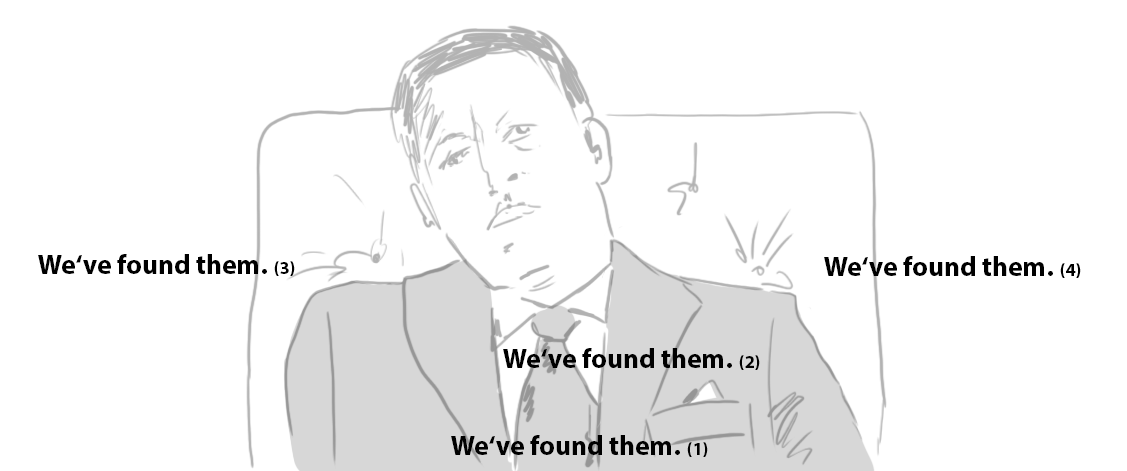
\includegraphics[width=\textwidth]{figures/FIG_39_nachbauen.png}}
\is{indicating speaking direction}
\caption{Examples for identified positions for off-screen speakers (sketch after a scene from \textit{Fast Five}): \\
1) Traditional (bottom-centre), 2) below focus (e.g. person spoken to), 3) next to focus, and 4) indicating speaking direction (e.g. speaker on the right outside the frame)}
\label{fig:FIG39}
\end{figure}

\figref{fig:FIG39} illustrates the derived positions for off-screen speakers. Besides the traditional position in the bottom-centre area (1), speakers and their \isi{speaking direction} can be indicated (4) or the titles placed below or next to the focus (2, 3).

\begin{figure}
\is{image composition}
\frame{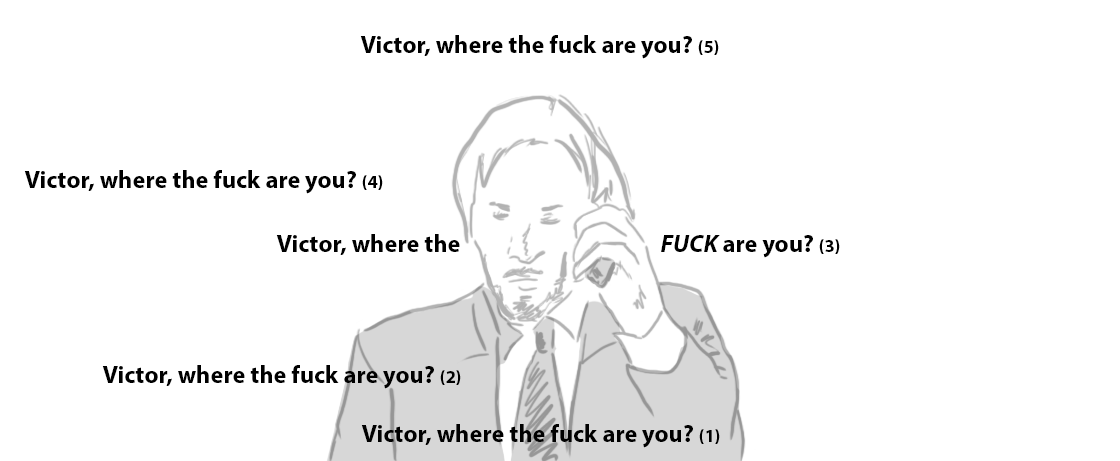
\includegraphics[width=\textwidth]{figures/FIG_40_nachbauen.png}}
\caption{Examples for identified positions for one visible speaker (sketch after a scene from \textit{John Wick}): \\
1) Traditional (bottom-centre) and below speaker, 2)  {speaking direction}, 3) around speaker, 4) next to speaker, and 5) above speaker. Other positions were effect-based (e.g. following an object or person through the frame) or based on the {image composition}.}
\label{fig:FIG40}
\end{figure}

\figref{fig:FIG40} shows the identified positions for visible speakers. Below (and alternatively above) the speaker (1, 5) allows for a quick identification. Indication of the \isi{speaking direction} (2) can be useful in conversations to allow for a quick focus change between speakers. The position next to a speaker (4) seems to be used in order not to cover important elements in the image, and the very specific position around the speaker in \textit{John Wick} (3) supports the central position of the speaker, allowing to focus on his face during the reading of the title.

  

\begin{figure}[b]
\frame{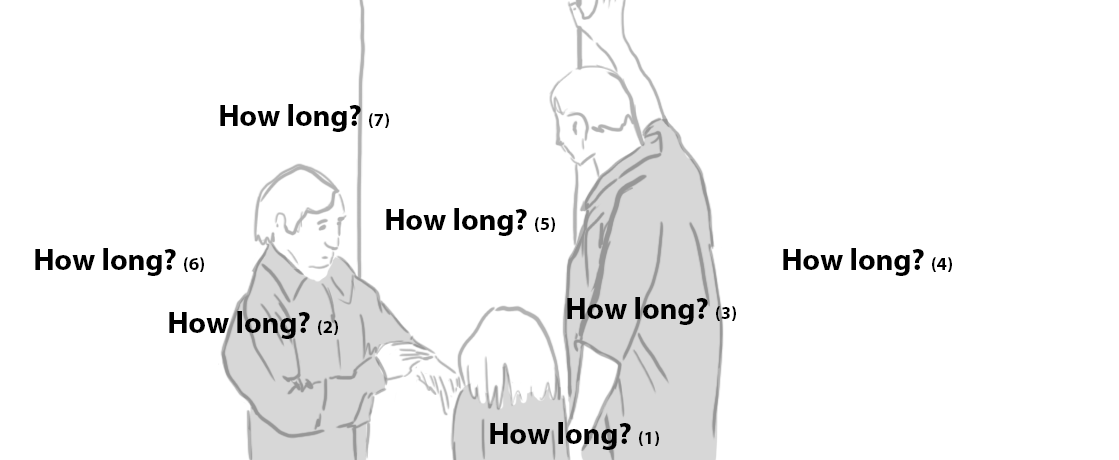
\includegraphics[width=\textwidth]{figures/FIG_41_nachbauen.png}}
\caption{Examples for identified positions for two or more visible speakers (sketch after a scene from \textit{Man on Fire}): 1) Traditional (bottom-centre), 2) below focus (e.g. person spoken to), 3) below speaker, 4) next to speaker, 5) in between speakers, 6) next to focus, and 7) above focus.}
\label{fig:FIG41}
\end{figure}

Finally, \figref{fig:FIG41} illustrates positions derived for two or more visible speakers. The first decisions seems to be whether the focus is supposed to be on the speaker or the person spoken to. Accordingly, titles were placed below speaker or focus (2, 3), in between them (5) or above (7). The positions next to speaker and focus (4, 6) again only seemed to be used in order not to cover important image areas or elements. The derived frequencies are listed in \tabref{tab:TAB11}.


\begin{sidewaystable}
\small
\begin{tabularx}{\textwidth}{lQrrrrrrrrrr>{\raggedleft}p{6mm}}
\lsptoprule
 Visible Speakers &  Placement Strategy &  MF &  ND &  H &  SM &  FF &  ST &  JW &  ALL &  \% &  Film count\\
 \midrule
Off-screen & Traditional (bottom) & 15 & - & 2 &  & 3 & - & - & 20 & 2.67 & 3\\
& Below focus & 18 & 2 & - & 3 & - & - & 9 & 32 & 4.28 & 4\\
& Next to focus & 22 & - & 3 & 12 & 14 & - & 1 & 52 & 6.95 & 5\\
& Speaking direction & - & - & 1 & 4 & - & 1 & - & 6 & 0.80 & 3\\
& Image composition & - & - & - & 7 & - & - & - & 7 & 0.94 & 1\\
1 Speaker & Traditional (bottom) & - & - & - & - & - & - & 5 & 5 & 0.67 & 1\\
& Around speaker & - & - & - & - & - & - & 3 & 3 & 0.40 & 1\\
& Below speaker & 54 & 8 & 51 & 33 & 16 & - & 12 & 174 & 23.26 & 6\\
& Next to speaker & 19 & - & 7 & 39 & 12 & - & 16 & 93 & 12.43 & 5\\
& Speaking direction & 54 & 14 & 16 & 23 & 13 & 7 & 3 & 130 & 17.38 & 7\\
& Effect-based & - & 15 & - & - & - & - & - & 15 & 2.01 & 1\\
& Image composition & - & - & - & 25 & - & - & - & 25 & 3.34 & 1\\
& Below focus & 1 & 17 & - & - & - & - & - & 18 & 2.41 & 2\\
2+ Speakers & Traditional (bottom) & - & - & - & - & - & - & 2 & 2 & 0.27 & 1\\
& Above focus & - & - & - & 1 & - & - & - & 1 & 0.13 & 1\\
& Below speaker & - & - & - & - & 27 & - & - & 27 & 3.61 & 1\\
& Below focus & 1 & - & - & 13 & - & - & - & 14 & 1.87 & 2\\
& Next to speaker & - & - & - & 16 & - & - & - & 16 & 2.14 & 1\\
& Next to focus & - & - & - & 12 & - & - & - & 12 & 1.60 & 1\\
& In between speakers\footnote{Includes ``\isi{speaking direction}''.} & 35 & - & 16 & 14 & 16 & - & 7 & 88 & 11.77 & 5\\
Television & Placed in television & - & 8 & - & - & - & - & - & 8 & 1.07 & 1\\
\midrule
 Integrated &  &  219 &  65 &  95 &  202 &  101 &  8 &  58 &  748 &  100.00 &  7\\
\tablevspace
 Traditional &  &  & 941 &  &  &  &  & 12 & 953 &  & 2\\
\lspbottomrule
\end{tabularx} 
\caption{Overview of all derived strategies for one visible speaker}
\label{tab:TAB11}
\end{sidewaystable}

As visible from \tabref{tab:TAB11}, \isi{placement} below the focus or \isi{focal point} in the image (e.g. a person spoken to or an object that is discussed) and next to a focus make up the biggest percentage of the derived strategies and were used in at least three of the six analysed films. The \isi{indication of speaking direction} can also be seen as relevant strategy as it was used in 50\,\% of the films. The indication of speaking directing for one visible speaker was used in all analysed films, followed by \isi{placement} below the speaker and next to the speaker. The derivation from this strategies is minimal (4.1\,\%) and only takes place in \textit{Slumdog Millionaire} where the titles do not seem to follow clear \isi{placement} strategies.

The only strategy for situations with two or more speakers used in more than two of the analysed films was the \isi{indication of speaking direction} which accounted for about 13\,\%. Even though a \isi{placement} close to the actual speaker seems like a favourable solution in scenes with multiple speakers and was in fact used for about 6.3\,\% of these titles, only one film made use of it. While a \isi{placement} close to a relevant object or \isi{focal point} might be a good solution, placing the title close to a person that is not the speaker might lead to confusion and misinterpretation of the scene (see \figref{fig:FIG42}) – especially for hearing-impaired audiences. This leads to the importance of defining an overall concept for the \isi{placement} strategies being used in the translation of a film with integrated titles and will be discussed in detail in \chapref{workflow} (workflow for the creation of integrated titles) and \chapref{method} (hypotheses and study).

\begin{figure}
\includegraphics[width=\textwidth]{figures/FIG42.jpg}
\caption{Title placed below the person spoken to despite the scene offering enough space for it to be placed under the actual speaker or in between speakers (\textit{Slumdog Millionaire}, 00:31:26)}
\label{fig:FIG42}
\end{figure}

In summary, the \isi{placement} strategies used in these analysed films are not as diverse as they might appear at first glance. For all of the three defined situations, three basic strategies can be defined due to their high frequency: below and next to a focus or speaker and \isi{indicating speaking direction} (as listed in \tabref{tab:TAB12}).

\begin{table}
\begin{tabularx}{\textwidth}{XX}
\lsptoprule
 Visible speakers &  Placement strategy\\
 \midrule
 Off-screen & Below focus\\
& Next to focus\\
& Speaking direction\\
 1 Speaker & Below speaker\\
& Next to speaker\\
& Speaking direction\\
 2+ Speakers & Below focus / speaker\\
& Next to focus / speaker\\
& In between speakers\\
\lspbottomrule
\end{tabularx}
\caption{Overview of all derived strategies with a high percentage and film count}
\label{tab:TAB12}
\end{table}

The result of this analysis is a first basic set of \isi{placement} strategies for integrated titles that can be extended by additional individual strategies such as the \isi{placement} around the speaker in \textit{John Wick} or those based on \isi{overall image composition} in \textit{Slumdog Millionaire}. These alternative positions for integrated titles, however, should only be used if this leads to a better processing and experience than the traditional \isi{placement} could offer. The goal of integrated titles should not be the use of alternative positions at all costs.

\section{Summary}\label{sec:4.3}

The ``interference'' of professionals from the film business without any background in translation and subtitling might have brought this industry on the long overdue new course towards a more integrated approach towards film translation and hopefully leads to better cooperation in the future. All in all, the derived strategies of the partially and completely integrated titles differ much less than might have been suspected. Noise transcriptions are placed below their source or indicate a source’s position outside the frame. The same goes for a combined title of \isi{noise transcription} and dialogue. Titles for off-screen speakers can be placed below a focus or \isi{focal point}, next to it or in \isi{indication of speaking direction}. One or more speakers offer placements below or next to the speaker, in \isi{speaking direction} and below or next to the focus in the image. As the titles created for the experiments discussed in the following chapters were created before some of these films even existed, they are not based on these entire findings but rather inspired by the older examples such as \textit{Man on Fire}, \textit{Slumdog Millionaire,} and \textit{Heroes}. The basic set of \isi{placement} strategies summarised here, however, is very relevant for the overall strategies and workflow model proposed in \chapref{workflow}.

The general recommendations for the creation of integrated titles developed in \sectref{sec:3.5} demand \isi{intuitiveness}, usefulness and satisfaction from titles. While it is difficult to rate the \isi{intuitiveness} of the mostly small amount of titles, the other two demands can be rated quite easily. Concerning usefulness, the translations seemed mostly suitable and readable. The \isi{eyestrain} was reduced in most cases due to small distances in between consecutive titles and most titles were placed close to the action and speakers. Concerning satisfaction (based on pleasant \isi{layout} and \isi{comprehensible design concept}), all titles appeared to be placed within the \isi{safe area}, used suitable typefaces and legible colour combinations and saturation. Shortcomings included very few incidents of unintended \isi{simultaneity}, the use of the rather weak top-centre position, collisions with relevant image areas, and a too long distance to the \isi{main focus}. While the SDH titles were mostly consistent concerning the \isi{placement} strategies, some films with integrated titles lacked consistency concerning both \isi{placement} and design and could therefore inflict irritation and reduced entertainment. As consistency is relevant for all three demanded characteristics of integrated titles, this can be seen as the most important lacking feature and the most serious shortcoming. If shortcomings are avoided and the general recommendations developed in \sectref{sec:3.5}, \sectref{sec:4.1.3}, and \sectref{sec:4.2.4} are followed, it is to be assumed that the individual \isi{placement} and design of integrated titles leads to better reception and increased \isi{entertainment value} of the respective film. Based on the so far presented theoretical framework, a basic workflow had to be developed to create the integrated titles for the reception study. This workflow and its application is presented in the following chapter.

